\section{第1章}

\subsection{题目1}

根据以下方法构造算法和MATLAB程序,以便精确计算所有情况下的二次方程的根,包括$|b| \approx \sqrt{b^2 - 4ac}$的情况。

\paragraph{分析}
~\\

设$a \neq 0, b^2 - 4ac > 0$,且有方程$ax^2 + bx + c = 0$,则通过如下二次根公式可解出方程的根:

\begin{equation}
x_1=\frac{-b+\sqrt{b^2-4ac}}{2a}  \quad \quad x_2=\frac{-b-\sqrt{b^2-4ac}}{2a}
\label{eq1}
\tag{1}
\end{equation}

通过将分子有理化,可以等价变换成下列公式

\begin{equation}
x_1=\frac{-2c}{b+\sqrt{b^2-4ac}} \quad \quad x_2=\frac{-2c}{b-\sqrt{b^2-4ac}}
\label{eq2}
\tag{2}
\end{equation}

当$|b| \approx \sqrt{b^2 - 4ac}$,必须小心处理,以避免其值过小而引起巨量消失(catastrophic cancellation)而带来精度损失。

\begin{itemize}
	\item 当$b > 0$的时候应使用公式(\ref{eq2})计算$x_1$,应使用公式(\ref{eq1})计算$x_2$。
	\item 当$b < 0$的时候应使用公式(\ref{eq1})计算$x_1$,应使用公式(\ref{eq2})计算$x_2$。
\end{itemize}

\paragraph{实验结果}
~\\[.5em]
\noindent 方程$x2+2.001x+1=0$: $x0=−0.968873270798,x1=−1.032126729202$.\\
方程$x2−1000.001x+1=0$: $x0=1000.000000000000,x1=0.001000000000$.\\
方程$x2−1000.0001x+1=0$: $x0=999.999099999100,x1=0.001000000900$.\\
方程$x2−1000.00001x+1=0$: $x0=999.999009999010,x1=0.001000000990$.\\
方程$x2−1000.000001x+1=0$: $x0=999.999000999001,x1=0.001000000999$.\\

\paragraph{代码}
~\\[.5em]
\begin{minted}{python}
def solve_quad(a, b, c):
    delta = b * b - 4 * a * c
    if delta < 0:
        return None 
    elif delta == 0:
        return [-b / (2 * a)]
    elif b > 0:
        return [-2 * c / (b + np.sqrt(delta)),
                (-b - np.sqrt(delta)) / (2 * a)]
    elif b < 0:
        return [(-b + np.sqrt(delta)) / (2 * a),
                -2 * c / (b - np.sqrt(delta))]

def disp_solve_quad(a, b, c):
    res = solve_quad(a, b, c)
    x = sp.Symbol('x')
    f = a * x * x + b * x + c
    if res is None:
        display(Math('方程 %s = 0 无解.' % sp.latex(f)))
    elif len(res) == 1:
\end{minted}

\begin{minted}{python}
        display(Math('方程 %s = 0 有一解: x = %.12f.' 
                     % (sp.latex(f), res[0])))
    else:
        display(
            Math('方程 %s = 0 有两解: x_0 = %.12f, x_1 = %.12f.'
                 % (sp.latex(f), res[0], res[1])))

disp_solve_quad(1, -1000.001, 1)
disp_solve_quad(1, -1000.0001, 1)
disp_solve_quad(1, -1000.00001, 1)
disp_solve_quad(1, -1000.000001, 1)
\end{minted}

\subsection{题目2}

对下列3个差分方程计算出前十个数值近似值。在每种情况下引入一个小的初始误差。如果没有初始误差,则每个差分方程将生成序列$\left\{1/2^n\right\}_{n=1}^\infty$,构造误差表和误差图。

\begin{enumerate}
	\item $r_0=0.994,r_n=\frac{1}{2}r_{n-1},n=1,2,\cdots$
	\item $p_0=1,p_1=0.497,p_n=\frac{3}{2}p_{n-1}-\frac{1}{2}p_{n-2},n=2,3,\cdots$
	\item $q_0=1,q_1=0.497,q_n=\frac{5}{2}q_{n-1}-q_{n-2},n=2,3,\cdots$
\end{enumerate}

\paragraph{基础知识:误差}
\begin{enumerate}
	\item 误差的来源
	由于计算机中二进制数精度有限, 存在截断误差(10进制与2进制互相转化, 2进制计算); 
	\item 误差的类型
	\subitem 截断误差: 通常指的是, 用一个基本表达式替换一个相当复杂的算术表达式时, 所引入的误差. 这个术语从用截断泰勒级数替换一个复杂表达式的技术衍生而来.
	\subitem 舍入误差: 计算机表示的示数受限于尾数的固定精度, 因此有时并不能确切地表示真实值, 这一类型的误差称为舍入误差.
	\item 误差度量方法: 
	设$\hat{p}$是$p$的近似值,
	\subitem 相对误差
	$$R_p = \frac{\left|p-\hat{p} \right|}{p}, p\neq 0$$
	\subitem 绝对误差
	$$E_p = \left|p - \hat{p}\right|$$
	\subitem 当$\left|p\right|$远离$1$时(大于或小于), 相对误差$R_p$比误差$E_p$能更好地表示近似值的精确程度.
\end{enumerate}

\paragraph{基础知识:误差的收敛阶}
~\\[.5em]
序列的收敛阶
设$\lim\limits_{n\to \infty}x_n = x$, 有序列$\left\{r_n \right\}_{n=1}^{\infty}$, 且$\lim\limits_{n \to \infty}r_n = 0$. 如果存在常量$K>0$, 满足
$\frac{\left|x_n - x\right|}{\left|r_n \right|} \leq K$, $n$足够大, 则称$\left\{ x_n\right\}_{n=1}^{\infty}$以收敛阶$O\left(r_n\right)$收敛于$x$.
可以将其表示为$x_n = x + O \left(r_n\right)$, 或表示为$x_n \to x$, 收敛阶为$O\left(r_n\right)$.
\paragraph{求解:生成序列}
~\\[.5em]
设$\{s_n\} = \left\{1/2^n\right\}_{n=1}^\infty$为标准序列,生成得到前10项序列值:

\begin{table}[H]
	\centering
	\caption{生成序列表}
	\begin{tabular}{cllll}
		\hline
		$n$ & \multicolumn{1}{c}{$s_n$} & \multicolumn{1}{c}{$r_n$} & \multicolumn{1}{c}{$p_n$} & \multicolumn{1}{c}{$q_n$} \\ \hline
		1   & 1.000000000000            & 0.994000000000            & 1.000000000000            & 1.000000000000            \\
		2   & 0.500000000000            & 0.497000000000            & 0.497000000000            & 0.497000000000            \\
		3   & 0.250000000000            & 0.248500000000            & 0.245500000000            & 0.242500000000            \\
		4   & 0.125000000000            & 0.124250000000            & 0.119750000000            & 0.109250000000            \\
		5   & 0.062500000000            & 0.062125000000            & 0.056875000000            & 0.030625000000            \\
		6   & 0.031250000000            & 0.031062500000            & 0.025437500000            & -0.032687500000           \\
		7   & 0.015625000000            & 0.015531250000            & 0.009718750000            & -0.112343750000           \\
		8   & 0.007812500000            & 0.007765625000            & 0.001859375000            & -0.248171875000           \\
		9   & 0.003906250000            & 0.003882812500            & -0.002070312500           & -0.508085937500           \\
		10  & 0.001953125000            & 0.001941406250            & -0.004035156250           & -1.022042968750           \\ \hline
	\end{tabular}
\end{table}

使用折线图将四个序列进行可视化,

\begin{figure}[H]
	\centering
	\caption{生成序列的折线图}
	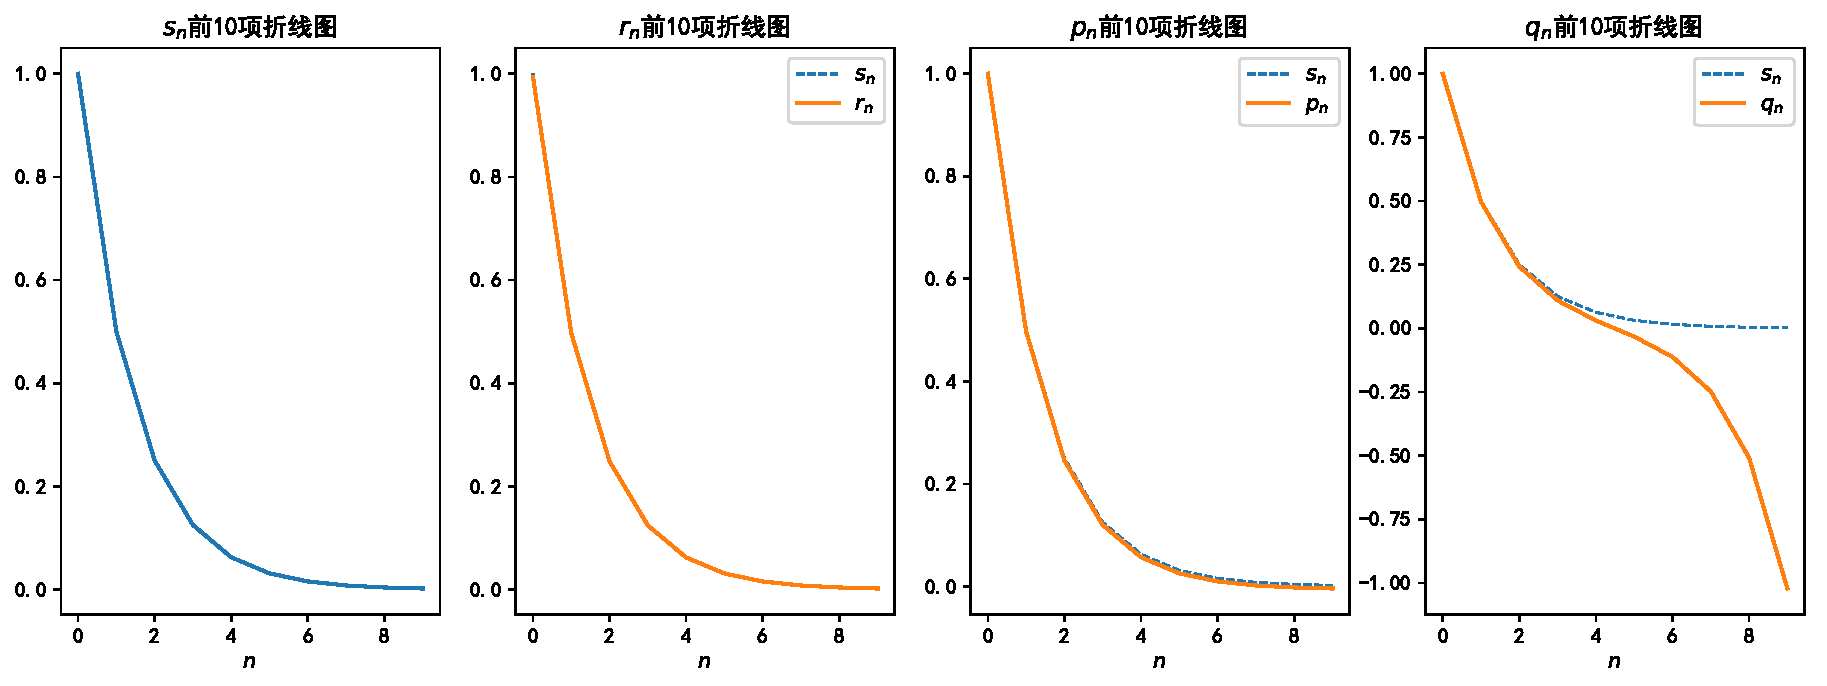
\includegraphics[width=\linewidth]{fig1.pdf}
\end{figure}

数列$\{s_n\}$与$\{r_n\}$,$\{p_n\}$,$\{q_n\}$之差的前10项:

\begin{table}[H]
	\centering
	\caption{生成序列误差表}
	\begin{tabular}{clll}
		\hline
		$n$ & \multicolumn{1}{c}{$s_n - r_n$} & \multicolumn{1}{c}{$s_n - p_n$} & \multicolumn{1}{c}{$s_n - q_n$} \\ \hline
		1   & 0.006000000000            & 0.000000000000            & 0.000000000000            \\
		2   & 0.003000000000            & 0.003000000000            & 0.003000000000            \\
		3   & 0.001500000000            & 0.004500000000            & 0.007500000000            \\
		4   & 0.000750000000            & 0.005250000000            & 0.015750000000            \\
		5   & 0.000375000000            & 0.005625000000            & 0.031875000000            \\
		6   & 0.000187500000            & 0.005812500000            & 0.063937500000            \\
		7   & 0.000093750000            & 0.005906250000            & 0.127968750000            \\
		8   & 0.000046875000            & 0.005953125000            & 0.255984375000            \\
		9   & 0.000023437500            & 0.005976562500            & 0.511992187500            \\
		10  & 0.000011718750            & 0.005988281250            & 1.023996093750            \\ \hline
	\end{tabular}
\end{table}

绘制每个序列的误差变化折线图,

\begin{figure}[H]
	\centering
	\caption{生成序列的误差变化折线图}
	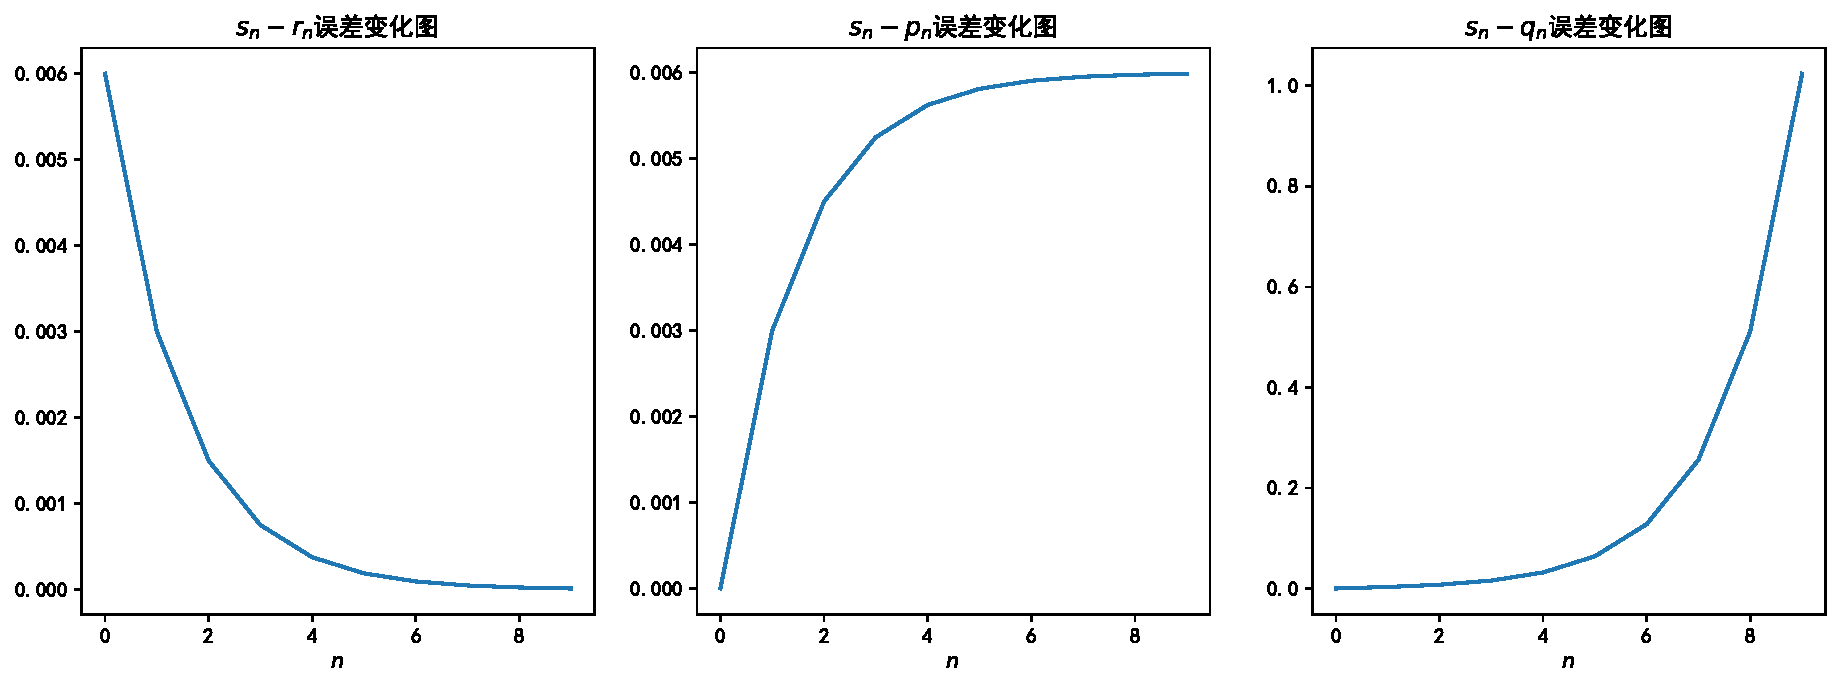
\includegraphics[width=\linewidth]{fig2.pdf}
\end{figure}

将其放在同一坐标系下,

\begin{figure}[H]
	\centering
	\caption{同一坐标系对比图}
	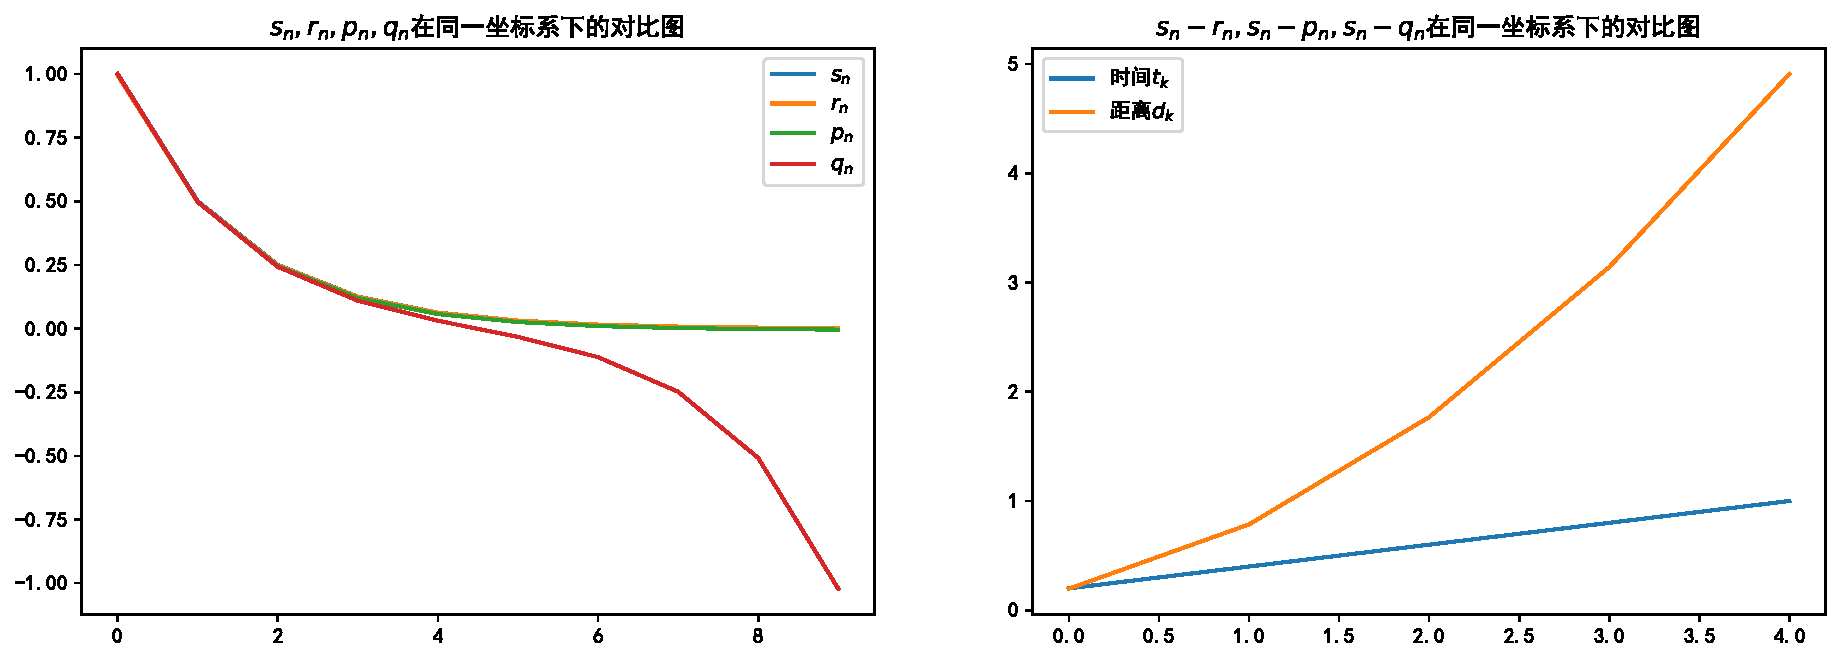
\includegraphics[width=\linewidth]{fig3.pdf}
\end{figure}

\paragraph{分析}
由图表可以发现$p_n$和$r_n$都可以较好地生成需要的序列,而$q_n$却随着$n$的增加离需要构造的序列真实值越来越远。
